\section{Results}
\label{section:results}

\subsection{Category Reduction}
\label{section:category-reduction}

\begin{table}
\centering
\begin{tabular}{@{}llll@{}}
  \toprule
  Layer $\alpha$ & Instances & Categories & \% Reduction \\
  \midrule
  0 & 2841 & 605 & 78.7 \\
  1 & 1738 & 601 & 65.4 \\
  2 & 824 & 438 & 46.8 \\
  3 & 356 & 319 & 10.3 \\
  \bottomrule
\end{tabular}
\caption{Category Reduction}
\label{table:category-reduction}
\end{table}

Looking at table \ref{table:category-reduction}, we see that at each layer, there is a reduction in the number of symbols represented at that abstraction level.  At level 0, we see the largest reduction from instances to categories of 78.7\%.  A large portion of this reduction is due to the categorization of 'silence' -- that is, inaudible white noise -- that, from moment to moment, has distinct values that are extremely close together in space.  This can be seen at the beginning of the clip in Figure \ref{figure:category-flow}.

As the level of abstraction increases, the number of instances in that layer decrease due to segmentation.  In addition, categorization still occurs at each level, though the degree at which instances are categorized together also decreases.  This is due most significantly to the 'silence' categories being hierarchically categorized together into fewer categories, though, as we will see in the following sections, other non-silence categories are being grouped together as well.

\subsection{Category Flow}
\label{section:category-flow}

\begin{figure}
  \centering
  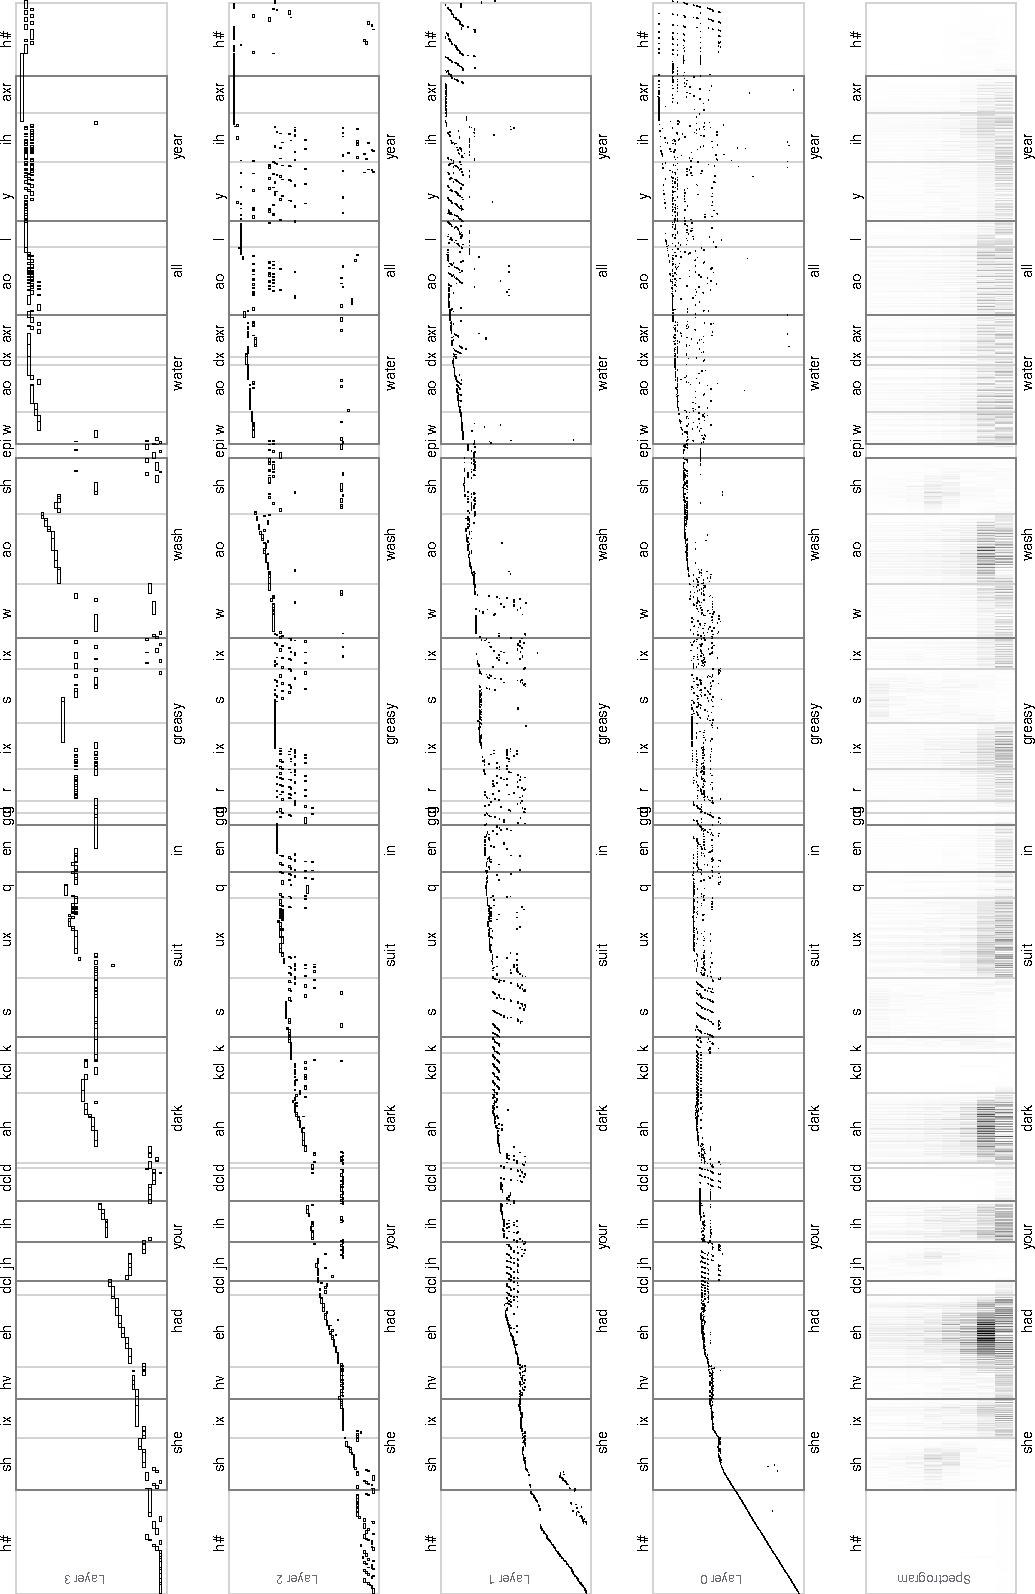
\includegraphics[width=\linewidth]{fig/category-flow-90.pdf}
  \caption{Category Flow of layers 0-3 with a Spectrogram}
  \label{figure:category-flow}
\end{figure}

The Category Flow diagram (Figure \ref{figure:category-flow}) illustrates the hierarchical categorization process. At each level, the word and syllable annotations boundaries are overlaid on top of the categories to easily discern where a certain sound should approximately begin and end.  The spectrogram is also displayed for visual comparison of the annotations and the actual signal.  In the category flow, each category is represented for its duration in the clip for each abstraction level, where each category has a spot on the y-axis -- that is, a category corresponds to a horizontal line on the plot.  In order to illustrate how transitions in a subordinate layer are abstracted into categories in the superordinate layer, the categories are ordered according to their maximum pair frequency such that categories that often appear in sequence are next to each other vertically.

In the category flow, we see that lower levels are quite noisy, with nearly all categories persisting for a single moment.  As we move up in abstraction, the flow flattens out and solidifies, meaning that trajectories from the subordinate layers are being categorized together in the superordinate layer.  As the abstraction level increases, we see a tendency for transitions between categories to flatten out into a smaller number of categories, where at the higher levels, these transitions flatten out completely into just one category.  By solidifying, we mean that the dispersed, noisy transitions found in the lower layers are categorized together in the upper layers, resulting in a "denser" category flow.

This process begins a bit in layer 2, but occurs much more frequently in layer 3.  This is most easily seen in the silent portion, marked \textit{h\#}, at the beginning of the clip.  Since this syllable is not actually silent because it contains faint white noise, the lower layers categorize these different moments of white noise separately, resulting in the ramp in categories at level 0.  Moving up the abstraction layers, their trajectories are categorized together into just a handful of categories at level 3.  This is evidence that the spectral representations of trajectories are consistently being categorized together if the trajectories they are representing are similar.

We can also see a few sections at level 3 where the categories or trajectories nearly line up with the syllable annotation boundaries.  For instance, the 's' syllable in the word 'suit' has been categorized into one category at this level, and the trajectory for the 'ao' syllable in the word 'wash' is clearly demarcated at the annotated boundaries.  One would expect that at the next level of abstraction, these trajectories would then become categories.

When examining all the abtractions layers as a whole, one can see noisy category transitions at the bottom layers become more consistent at the upper layers.  Even more, we can see that similar trajectories in lower layers are categorized together in upper layers.  This is evident in the 'striping' seen in lower layers -- perhaps a frequency beating artifact of the recording -- becoming a single category in upper layers.  This is seen most readily in the 's' syllable of the word 'suit', which exhibits striping at the lower levels.  Since these transitions are very similar, their trajectories and therefore spectral representations should be similar. Indeed, we see that at the upper levels these similar transitions are all categorized together, indicating that the categorization of spectral representations of trajectories behaves as expected as outlined in the theory.

\subsection{Category Distribution}
\label{section:category-distribution}

\begin{figure}
  \centering
  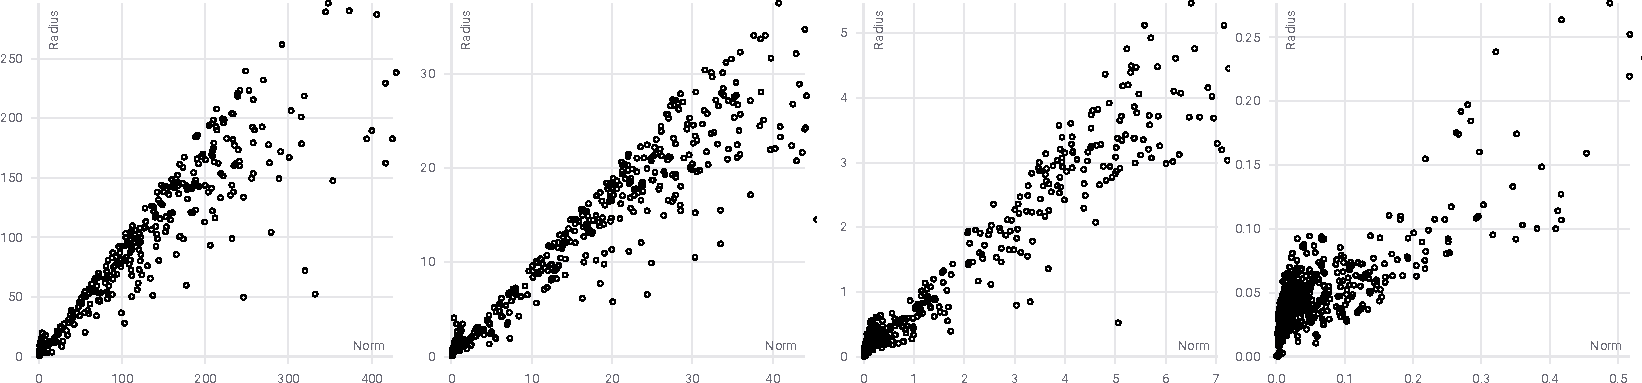
\includegraphics[width=\linewidth]{fig/category-distribution.pdf}
  \caption{Category Distribution of layers 0-3 going from right to left}
  \label{figure:category-distribution}
\end{figure}

 Since, especially at the higher levels, visualizing these high-dimensional categories is nigh impossible, the category distributions plot (figure \ref{figure:category-distribution}) shows the distribution of categories for a given dimension by showing how far away a given category is from the origin (i.e. the norm of the centroid of a category) on the x-axis, and the radius of the category on the y-axis.  This means points to the right of the distribution represent categories that are in general more distant from other categories, and points toward the top will have a larger inclusion radius $\rho$ and volume.

Looking at all of the distributions, one can immediately see a positive correlation between the remoteness (i.e. distance from the origin) of a category and its volume.  At each abstraction level, we see most categories are close together with a small volume, and as they move away from the origin, there volume also increases.  This is to be expected since the adaptive categorization tends to reduce the volume of categories with many members, and there are more instances near the origin than away from it.  Therefore, looking at the space as a whole, we see that the category density is high near the origin, and more sparse as one moves out.

It is also important to note that the adaptive categorization method employed here is not overly constraining the radii of each dimension.  If it were, instead of the linear trend we see here, the trend would shoot up to initial radius $\rho_0$ of the dimension and flatten out in an inverted-L shape.  This top-flattening not only results in most categories having nearly the same volume, but would also result in a larger amount of non-categorizable regions in the space; both of these qualities are undesirable.  In fact, the maximum posterior radius for each level is well below the initial radius, indicating that it is not a limiting factor in the categorization.  This shows that the adaptive categorization fills the space quite well, though more analysis would need be done to determine the analytical extent of the spatial covering, left to future research.

\subsection{Category Similarity}
\label{section:category-similarity}

\begin{figure}
  \centering
  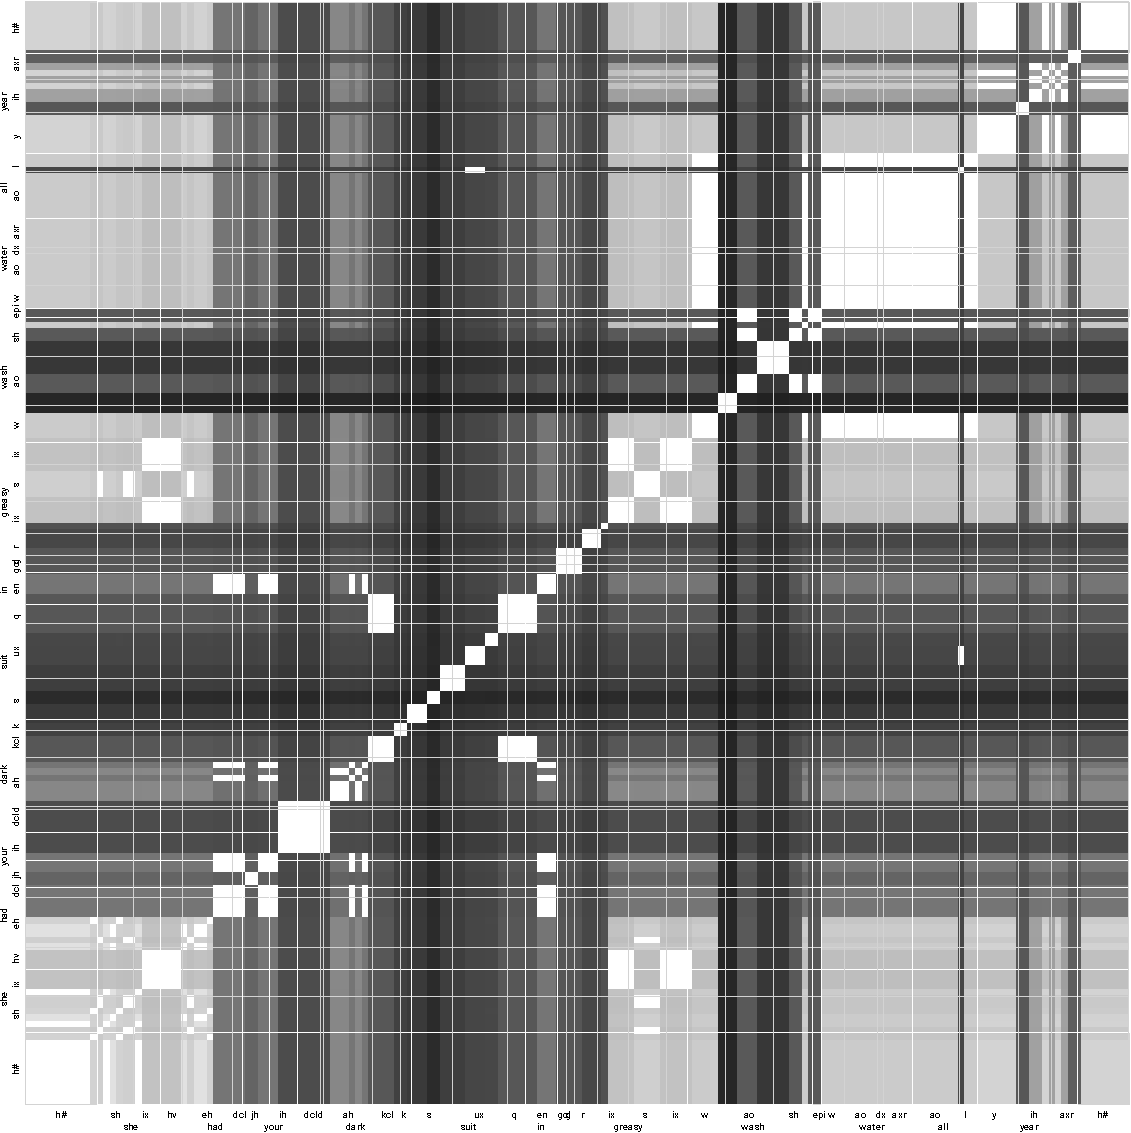
\includegraphics[width=\linewidth]{fig/category-similarity-90.pdf}
  \caption{Category Similarity of Abstraction Layer 3}
  \label{figure:category-similarity}
\end{figure}

Since it is difficult to discern in the category flow (figure \ref{figure:category-flow}) if there is consistent categorization of similar sounds across the whole clip, the category similarity matrix (figure \ref{figure:category-similarity}) for abstraction level $\alpha = 3$ can be used instead.  At each moment in the clip the current category is compared with the category of every other moment in the clip, finding their distance, and representing closer categories with lighter shades and distant categories with darker shades.  Therefore, we see that diagonal is white, since the category of a moment has zero distance to itself.  Both axes of the matrix are also annotated with the words and syllables, like in the category flow, so that the similarity between different words and syllables of the clip can be compared.

Looking for light areas off the diagonal, there are three main areas of interest.  The first is at the intersection of 'she' and 'greasy'.  Clearly, the syllables of these words sound similar, so it makes sense that this area is lightly shaded and white.  Another white area is at the intersection of the words 'had' and 'in'.  Though in most accents these syllables of these words sounds quite different, the particular New England accent of this speaker has these words sounding similar -- something near 'hed' and 'en'. The other off-diagonal white area to call out comes at the intersection at the end of the words 'dark' and 'suit'.  For this accent, the ends of both of these words are unpronounced and are replaced with a stop, meaning they also qualitatively sounds quite similar.

Since similar sounding syllables are either in the same category or very close categories, this is evidence that categories semantically representing human speech syllables are beginning to emerge at this level.  Note that this emergence is occurring without any knowledge of this domain being human speech data, meaning that the general IDyOT processes behave as expected without specifying domain-specific information in the model.
